\documentclass{beamer}
\usetheme[shownavsym]{AAUsimple}
\usefonttheme{structurebold}
%%%%%%%%%%%%%%%%%%%%%%%%%%%%%%%%%%
\usepackage[utf8]{inputenc}
\usepackage[dutch]{babel}
\usepackage[T1]{fontenc}
\usepackage{tikz}
\usepackage{hyperref}
\usepackage{lmodern}
\usepackage{microtype}
%%%%%%%%%%%%%%%%%%%%%%%%%%%%%%%%%%
% Gekleurde hyperlinks
\newcommand{\chref}[2]{%
	\href{#1}{{\usebeamercolor[bg]{AAUsidebar}#2}}%
}
\title[Immunologie]{Complement systeem}

\date{\today}

\author[Edon Namani, et. al]
{%
	Edon Namani\\
	\href{mailto:e.namani@student.rug.nl}{{\tt e.namani@student.rug.nl}}
}

\institute[%
	Faculteit Gezondheidswetenschappen\\
	Rijksuniversiteit Groningen\\
	Nederland
]
{%
	Faculteit Gezondheidswetenschappen\\
	Rijksuniversiteit Groningen\\
	Nederland

}

\pgfdeclareimage[height=1.5cm]{titlepagelogo}{AAUgraphics/semper_invicta.pdf}
\begin{document}
% Titel
{\aauwavesbg%
	\begin{frame}[plain,noframenumbering]
	\titlepage
\end{frame}}
%%%%%%%%%%%%%%%

%TOC
\begin{frame}{Agenda}{}
	\tableofcontents
\end{frame}
%%%%%%%%%%%%%%%
\section{Functies van complement systeem}
\begin{frame}{Functies van complement systeem}
	\begin{enumerate}
		\item Promotie van ontsteking.
		\item Opsonisatie $\rightarrow$ het proces waarbij anti-genen worden getagd. Tagging van de antigenen bevordert fagocytose.
		\item Cel-lysis
	\end{enumerate}
\end{frame}

\section{Analogie stolling en complement systeem}
\begin{frame}
	\begin{block}{Analogie Stolling en complement systeem}
		Het complement systeem is vergelijkbaar met de stolling. Zoals in stolling heb je ook in het complement systeem ongeactiveerde proteolytische enzymen. Door een trigger wordt een proteolytische cascade gestart. Deze trigger is hechting van oplosbare eiwitten aan antigenen.
	\end{block}
\end{frame}

\section{Initiators van complement cascade}
\begin{frame}{De Triggers}
	\begin{columns}
	\begin{column}{.5\textwidth}
	\begin{enumerate}
		\item C1-prote\"ine \& immunoglobuline complex
		\item Collectin(MBL)
		\item Ficolin
		\item Acute-fase prote\"ine, zoals CRP
	\end{enumerate}
\end{column}
%%%
\begin{column}{.5\textwidth}
	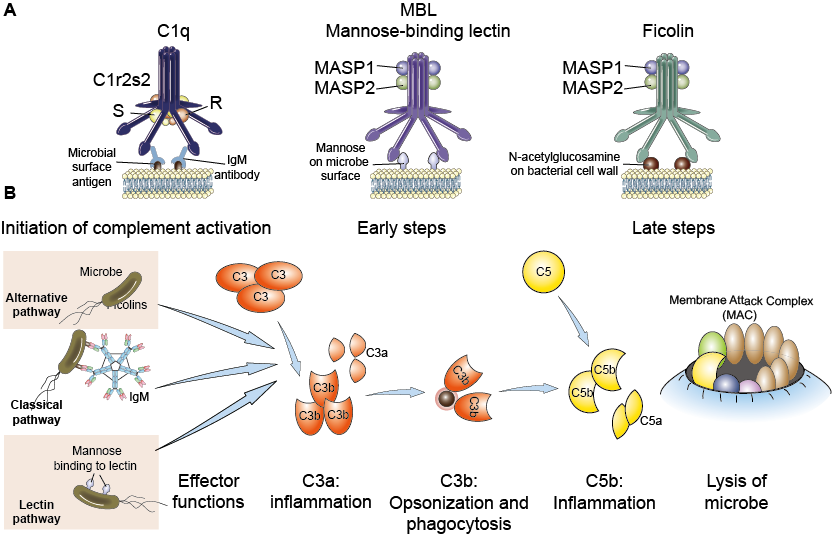
\includegraphics[width=\textwidth]{complement.png}
\end{column}
\end{columns}
\end{frame}

{\aauwavesbg
\begin{frame}[plain,noframenumbering]
	\finalpage{Bedankt voor het aandachtig luisteren!}
\end{frame}}
\end{document}
